\section*{Problem 4}

Find the response of the following systems to the input below. 
Sketch the magnitude of each frequency
response for $-\pi< \omega <\pi$ and determine the type of filter.

$x[n] = 2 + 2\cos(n \pi/4) + \cos(n 2\pi /3 + \pi/2)$

\begin{itemize}
\item $H(\omega) = e^{-j \omega} \cos(\omega/2)$
\end{itemize} 
\subsection*{Solution}

\begin{equation*}
\begin{aligned}
X(\omega) &= 4\pi \delta(\omega) + 
	2 \pi [\delta(\omega - \frac{\pi}{4}) + \delta(\omega + \frac{\pi}{4})] +
	  \pi [\delta(\omega - \frac{2 \pi}{3}) + \delta(\omega + \frac{2 \pi}{3})]
\end{aligned}
\end{equation*} 

\zcodemat{sources/c4p4a.m}{Magnitud y Fase de los espectros de las señales}

\begin{figure}[H]
\caption{Plot for $H(\omega)\; X(\omega)\; Y(\omega)$}
\centering
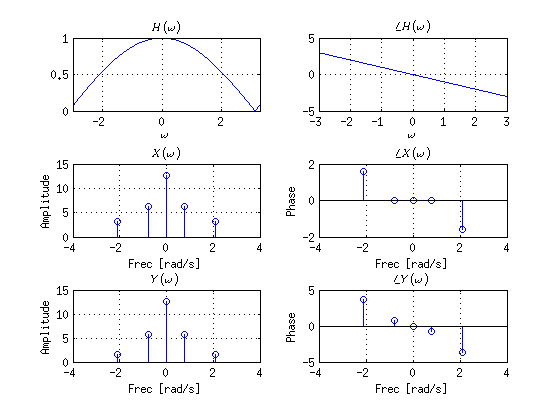
\includegraphics[width=0.8\textwidth]{figs/c4p4a.png}
\label{fig:c4p4a}
\end{figure} 

Output signal spectra is obtained by multiplying $X(\omega)$ with $H(\omega)$ as
can be seen in figure \ref{fig:c4p4a}. The values of the filter that multiplies
the magnitudes of the input can be obtained by evaluating $H$ in each of 
the frecuencies were the delta function appears.

Also, H is a low-pass filter as can be seen in the spectra. The
output function is given by:

\begin{equation*}
\begin{aligned}
y[n] &= (1)(2) + (0.9239)(2)\cos(n \pi/4 - \pi/4) + (0.8660) \cos(n 2\pi/3 - \pi/6 ) \\
     &= 2 + 1.85 \cos(n \pi/4 - \pi/4) + 0.87 \cos(n 2\pi/3 - \pi/6 ) \\
\end{aligned}
\end{equation*}

\begin{itemize}
\item $H(\omega) = e^{-j \omega / 2} (1 - \cos(\omega/2))$
\end{itemize} 
\subsection*{Solution}

\zcodemat{sources/c4p4b.m}{Magnitud y Fase de los espectros de las señales}

\begin{figure}[H]
\caption{Plot for $H(\omega)\; X(\omega)\; Y(\omega)$}
\centering
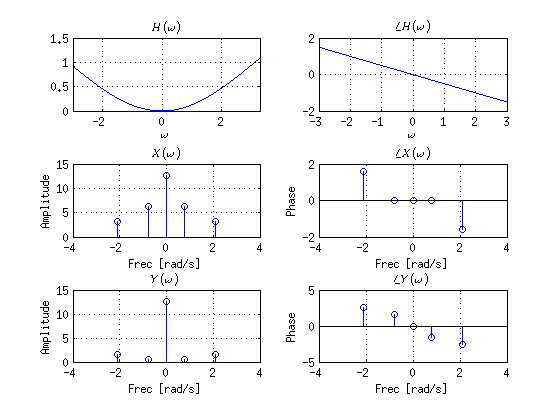
\includegraphics[width=0.8\textwidth]{figs/c4p4b.png}
\label{fig:c4p4b}
\end{figure} 

Output signal spectra is obtained by multiplying $X(\omega)$ with $H(\omega)$ as
can be seen in figure \ref{fig:c4p4a}. The values of the filter that multiplies
the magnitudes of the input can be obtained by evaluating $H$ in each of 
the frecuencies were the delta function appears.

Also, H is a high-pass filter as can be seen in the spectra so the
constant frecuency will be filtered out. 
The output function is given by:

\begin{equation*}
\begin{aligned}
y[n] &= 0.15 \cos(n \pi/4 - \pi/8) + 0.5 \cos(n 2\pi/3 + \pi/6 ) \\
\end{aligned}
\end{equation*} 
